\documentclass{beamer}
\usepackage[utf8]{inputenc}
\usepackage{amsthm}
\usepackage{amsmath}
\usepackage{graphicx}
\usetheme{Copenhagen}
\title{Matrix Problem}
\author{Karthik and Abhishek}
\institute{IIT Hyderabad}

\begin{document}
\begin{frame}
\titlepage    
\end{frame}
\begin{frame}{Contents}
\tableofcontents
\end{frame}
\section{Geometric Question}
\begin{frame}{Geometric Question}
Let k be an integer such that the triangle with vertices
(k,-3k),(5,k),(-k,2)
has area 28. Find the orthocentre of this triangle.    
\end{frame}
\section{Matrix Transformation of Geometric Question}
\begin{frame}{Matrix Transformation Of Geometric Question}
Let k be an integer such that the triangle with vertices
$\begin{bmatrix} k \\ -3k \end{bmatrix}$,
$\begin{bmatrix} 5 \\ k \end{bmatrix}$,
$\begin{bmatrix} -k \\ 2 \end{bmatrix}$
has area 28. Find the orthocentre of this triangle.
\end{frame}
\section{Solution In Form Of Matrix}
\begin{frame}{Solution In Form Of Matrix}
Area of triangle is 28
\\~\\
\begin{proof}{\textbf{NOTE:}}
	{
    \\
    Area of triangle of A
    $\begin{bmatrix} x1 \\ y1 \end{bmatrix}$,B
    $\begin{bmatrix} x2 \\ y2 \end{bmatrix}$,C
    $\begin{bmatrix} x3 \\ y3 \end{bmatrix}$ is
    $1/2 \times$
    $\begin{Vmatrix} x1 & y1 & 1 \\ x2 & y2 & 1 \\ x3 & y3 & 1 \end{Vmatrix}$
    }
\end{proof}
%\\
So,
\[\begin{Vmatrix} k & -3k & 1 \\ 5 & k & 1 \\ -k & 2 & 1 \end{Vmatrix} = 56\]
\end{frame}
\begin{frame}{Solution In Form Of Matrix}
\[5k^2 + 13k + 10 = 56 \Rightarrow 5k^2 + 13k - 46 = 0\] 
\
\[(OR)\]
\
\[5k^2 + 13k + 10 = -56 \Rightarrow 5k^2 + 13k + 66 = 0\]
\begin{proof}{\textbf{NOTE:}}
    {
    \\
    The roots of quadratic equation \(ax^2 + bx + c\) are: 
    \[x=\frac{-b\pm\sqrt{b^2-4ac}}{2a}\].
    }
\end{proof}
\end{frame}
\begin{frame}{Solution In Form Of Matrix}
On solving the above equations:
\[k = -4.6, 2, -1.3+3.39i, -1.3-3.39i\]
Since, k takes only integer values
\[\Rightarrow\textbf{k = 2}\].
The vertices of the triangle are:
\\
\[A
\begin{bmatrix} 2 \\ -6 \end{bmatrix},B
\begin{bmatrix} 5 \\ 2 \end{bmatrix},C
\begin{bmatrix} -2 \\ 2 \end{bmatrix}\]
\end{frame}
\begin{frame}{Solution In Form Of Matrix}
To calculate the foot of perpendicular from A to BC
\\
Let, $K_{1} = Normal-Vector-To-BC$
\\
     $K_{2} = Directional-Vector-Of-BC$
\\
Then:
\[K_{1}^T(X - B) = 0\]
\\
\[K_{2}^T(X - A) = 0\]    
\\
\[\Rightarrow
\begin{bmatrix}K_{1}^T \\ K_{2}^T \end{bmatrix}X = \begin{bmatrix}K_{1}^TB \\ K_{2}^TA \end{bmatrix}\]
\end{frame}
\begin{frame}{Solution In Form Of Matrix}
Then,
\\
\[X = \begin{bmatrix}K_{1}^T \\ K_{2}^T \end{bmatrix}^{-1}\begin{bmatrix}K_{1}^TB \\ K_{2}^TA \end{bmatrix}\]
\\
On solving we get:
\[P = \begin{bmatrix}2 \\ 2 \end{bmatrix}\]
\\
Similarly the other coordinates are:
\[Q = \begin{bmatrix}-0.6 \\ -0.8 \end{bmatrix}\]
\\
\[R = \begin{bmatrix}4.13 \\ -0.30 \end{bmatrix}\]
\end{frame}
\begin{frame}{Solution In Form Of Matrix}
To solve the intersection point of the Altitudes AP \& CR:
\\
Let,
$N_{1} = {Normal-Vector-To-AP}$
\\
$N_{2} = {Normal-Vector-To-CR}$
\\
Then:
\[N_{1}^T(X - A) = 0\]
\\
\[N_{2}^T(X - C) = 0\]    
\\
\[\Rightarrow
\begin{bmatrix}N_{1}^T \\ N_{2}^T \end{bmatrix}X = \begin{bmatrix}N_{1}^TA \\ N_{2}^TC \end{bmatrix}\]

\end{frame}
\begin{frame}{Solution In Form Of Matrix}
Then,
\\
\[X = \begin{bmatrix}N_{1}^T \\ N_{2}^T \end{bmatrix}^{-1}\begin{bmatrix}N_{1}^TA \\ N_{2}^TC \end{bmatrix}\]
\\
On solving we get:
\[H = \begin{bmatrix}2 \\ 0.5 \end{bmatrix}\]
\end{frame}
\begin{frame}{Figures}
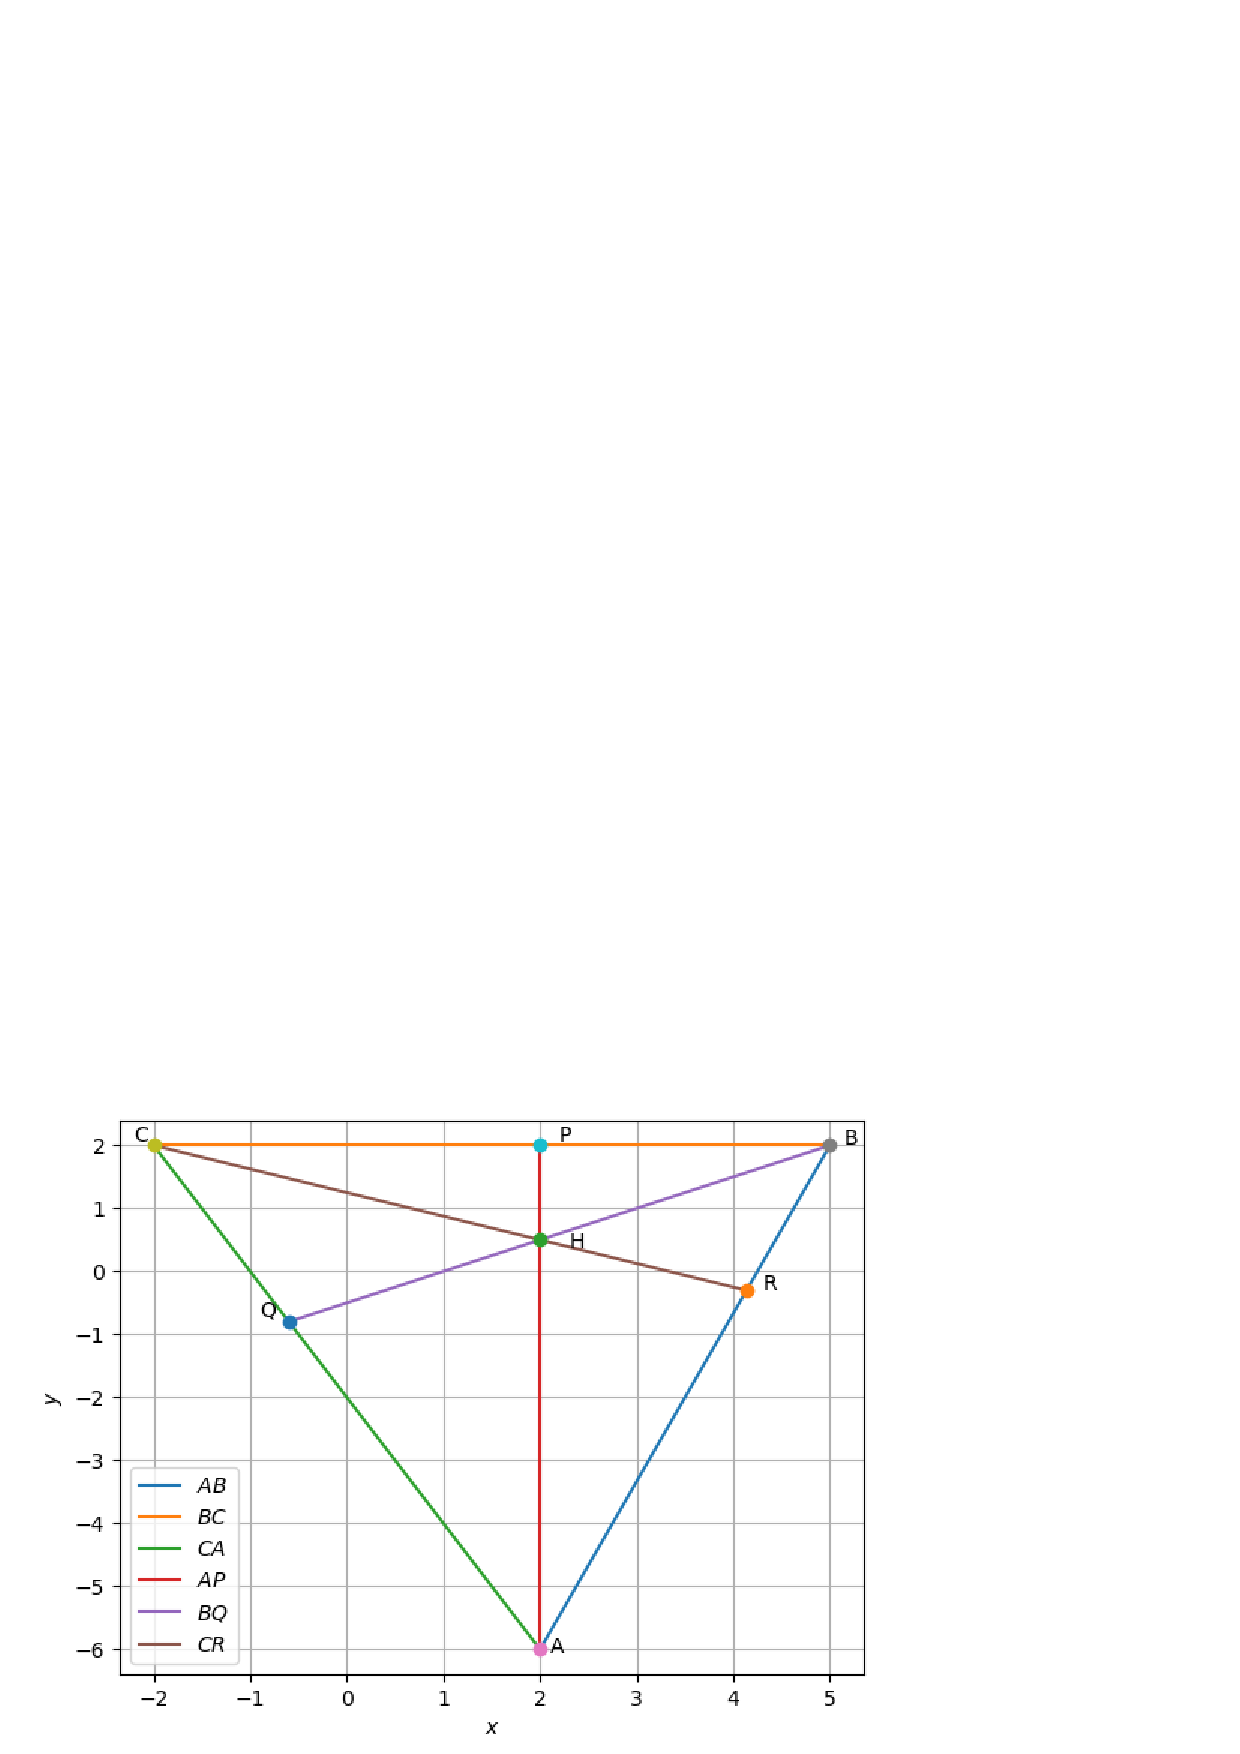
\includegraphics[scale = 0.6]{triangle.png}
\end{frame}
\end{document}